% chapter 3
\chapter{Requirements and Analysis}
In this chapter, we will focus on creating the LP formulations and identifying the requirements to solve the given problem.

\section{Problem Definition}
In one busy day, the company is scheduled to make deliveries to 226 customers across the country. The deliveries are made to the customers' location by delivery vehicles. All vehicles are
expected deliver all of the customers' goods in one visit.  There are 16 of these vehicles and they are based in
one central location (depot), where the company's goods are stored. The delivery vehicles only operate on
a time window from 09:00 to 17:00. On each delivery to a customer, it takes an average of 15 minutes for the workers to successfully unload the goods.
The company wants to find the routes that yield the minimum (optimal) distance and such that all customers are visited only once. They are interested
in finding the vehicle routes that yield the minimum distance for both with and without the time windows.
The company also wants to find out if it can use less vans to make all deliveries while
keeping the total distance roughly the same (or less) as deliveries with 16 vehicles. The vehicles may serve up to 50 customers in a single tour.

We may make the following assumptions for convenience in modelling the LP formulations:
\begin{enumerate}
\item The service time for all deliveries is set to 15 minutes.
\item All delivery vehicles are homogeneous and have very large capacity (up to 50 items).
\item Customers must receive all of their goods in a single visit, so we may set all customers' demand to 1.
\item The cost function is set to the distance travelled.
\item Distance from one point to another may be calculated using the euclidian formula. We may use the haversine
formula\footnote{See \url{https://en.wikipedia.org/wiki/Haversine_formula}} to get real distance in km.
\item Traffic conditions are negligible and we assume that the roads from one point to another are straight. We make this
assumption due to lack of data.
\end{enumerate}

In addition to solving their vehicle routing problem,  the company would like to compare popular LP tools
 so that they may use the one that suits their needs. To accomplish this, we should conduct a performance analysis on the chosen LP tools
and analyse their respective features.

\section{Mathematical Formulation}
We can specifically define the problem given in the previous section with two known VRP models: capacitated
vehicle routing problem (CVRP) \cite{Daneshzand2011} and capacitated vehicle routing problem
with time windows model (CVRPTW) \cite{Daneshzand2011, Desrochers1988}, both of which has a single depot.

The CVRP model has the following input:
\begin{itemize}
\item A complete graph \(G = (V, E)\). which consists of the vertices \(V\) and the edges \(E\).
\item The variable \(n\), which represent the total number of customers and the depot.
\item The variable \(K\), which represent the total number of vehicles available. This will dictate the number of routes
generated in the model, with each vehicle having its own route.
\item A vertex set \(V\), numbered from 1 to \(n\) and vertex 1 is the depot.
\item A set of edges for \(V\).
\item The cost function \(c_{ij}\) that outputs the distance travelled from vertex i to j, where \(i,j \in V\).
\item The path function \(x_{ij}\) that outputs 1 if the path i to j is included in the current journey and 0 otherwise.
\item The capacity function \(r(S)\) that outputs the number capacity needed to serve a set of customers \(S\).
\end{itemize}

Given the input above, we can create a single depot capacitated vehicle routing problem below:

\vspace{0.5cm}

\begin{equation}
    \begin{array}{ll@{}ll}
        \text{Minimize} & \displaystyle\sum\limits_{i \in V}\sum\limits_{j \in V} c_{ij}&x_{ij} &\\
    \end{array}
\end{equation}
\begin{equation}
    \begin{array}{ll@{}ll}
        \text{Subject to}&\displaystyle\sum\limits_{i \in V}   &x_{ij} = 1,  &\forall j \in V \setminus \{1\}\\
    \end{array}
\end{equation}
\begin{equation}
    \begin{array}{ll@{}ll}
        & \displaystyle\sum\limits_{j \in V}   &x_{ij} = 1,  &\forall i \in V \setminus \{1\}\\
    \end{array}
\end{equation}
\begin{equation}
    \begin{array}{ll@{}ll}
        & \displaystyle\sum\limits_{i \in V}   &x_{1i} = K\\
    \end{array}
\end{equation}
\begin{equation}
    \begin{array}{ll@{}ll}
        & \displaystyle\sum\limits_{i \in V}   &x_{i1} = K\\
    \end{array}
\end{equation}
\begin{equation}
    \begin{array}{ll@{}ll@{}ll}
        & \displaystyle\sum\limits_{i \in S}\sum\limits_{i \in S}  &x_{ij} \leq |S| - r(S), &\forall S \subseteq V/ \{1\} , S \neq \oldemptyset \\
    \end{array}
\end{equation}
\begin{equation}
    \begin{array}{ll@{}ll@{}ll}
        & x_{ij} = \{0,1\}\\
    \end{array}
\end{equation}

\vspace{1cm}

Equations (3.2) and (3.3) are constraints to ensure that all cities are visited only once, excluding the depot. Constraints (3.4) and (3.5)
impose the vehicles coming in must be equal to the vehicles coming out of the depot. Constraint (3.6) is the Subtour
Elimination Constraint (SEC) to ensure that each route is a hamiltonian cycle. This is to ensure that routes are optimal
 and accurately represent the situation in real life. Subtours are
cycles that exists within a set of vertices that partition the set into two or more components. Figures
3.2 and 3.3 illustrates the difference between a graph with subtours and a graph with a hamiltonian cycle.
\vspace{0.5cm}
\begin{figure}[!ht]
  \centering
    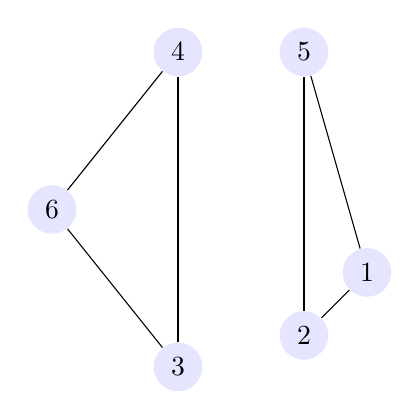
\begin{tikzpicture}
          [scale=.4,every node/.style={circle,fill=blue!10}]
          \node (n6) at (1,10) {6};
          \node (n4) at (5,15)  {4};
          \node (n5) at (9,15)  {5};
          \node (n1) at (11,8) {1};
          \node (n2) at (9,6)  {2};
          \node (n3) at (5,5)  {3};

          \foreach \from/\to in {n6/n4,n5/n1,n1/n2,n2/n5,n3/n4,n6/n3}
            \draw (\from) -- (\to);

        \end{tikzpicture}

      \caption{A graph with subtours}
      \label{fig:subtour}
\end{figure}

\begin{figure}[!ht]
  \centering
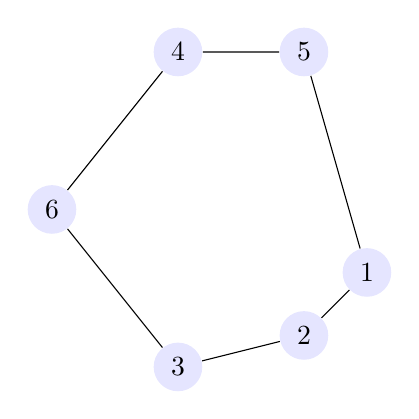
\begin{tikzpicture}
          [scale=.4,every node/.style={circle,fill=blue!10}]
          \node (n6) at (1,10) {6};
          \node (n4) at (5,15)  {4};
          \node (n5) at (9,15)  {5};
          \node (n1) at (11,8) {1};
          \node (n2) at (9,6)  {2};
          \node (n3) at (5,5)  {3};

          \foreach \from/\to in {n6/n4,n5/n1,n4/n5,n1/n2,n6/n3,n3/n2}
            \draw (\from) -- (\to);

        \end{tikzpicture}
      \caption{A graph with a hamiltonian cycle}
      \label{fig:hamiltoniancycle}
\end{figure}


There are two common formulations to eliminate subtours: the MTZ formulation by Miller \cite{Miller1960} and
the Subtour Formulation \cite{Lawler1985, Pataki2003}. Pataki \cite{Pataki2000} states that Subtour Elimination is the efficient formulation to reach optimal solution, whereas
the MTZ Formulation is highly inefficient despite its elegance. We formulate constraint (3.6) by combining capacity cut constraint (CCC), a constraint to ensure
that the vehicles meet the demands of all customers in a tour, with the Subtour Formulation to get the SEC for VRP \cite{Daneshzand2011}.

In order to model CVRPTW, we need to introduce a new set of input related to time window constraints:
\begin{itemize}
\item Variable \(D_{i}\) that represents the departure time to customer \(i\).
\item Time function \(t_{ij}\) that outputs the time taken to travel to customer \(i\) to \(j\).
\item Variable \(e_{i}\) that represents the earliest time for visiting customer \(i\).
\item Variable \(l_{i}\) that represents the latest time for visiting customer \(i\).
\item Variable \(y_{i}\) that represents the remaining capacity of the vehicle when visiting customer \(i\).
\item Variable \(q_{i}\) that represents the demand of customer \(i\).
\item Variable \(Q\) that represent the capacity of the vehicle \(i\).
\end{itemize}

Putting it together, we have the complete CVRPTW model below:

\vspace{0.5cm}

\begin{equation}
    \begin{array}{ll@{}ll}
        \text{Minimize} & \displaystyle\sum\limits_{i \in V}\sum\limits_{j \in V} c_{ij}&x_{ij} &\\
    \end{array}
\end{equation}
\begin{equation}
    \begin{array}{ll@{}ll}
        \text{Subject to}&\displaystyle\sum\limits_{i \in V}   &x_{ij} = 1,  &\forall j \in V \setminus \{1\}\\
    \end{array}
\end{equation}
\begin{equation}
    \begin{array}{ll@{}ll}
        & \displaystyle\sum\limits_{j \in V}   &x_{ij} = 1,  &\forall i \in V \setminus \{1\}\\
    \end{array}
\end{equation}
\begin{equation}
    \begin{array}{ll@{}ll}
        & \displaystyle\sum\limits_{i \in V}   &x_{1i} = K\\
    \end{array}
\end{equation}
\begin{equation}
    \begin{array}{ll@{}ll}
        & \displaystyle\sum\limits_{i \in V}   &x_{i1} = K\\
    \end{array}
\end{equation}
\begin{equation}
    \begin{array}{ll@{}ll@{}ll}
        & \displaystyle\sum\limits_{i \in S}\sum\limits_{i \in S}  &x_{ij} \leq |S| - r(S), &\forall S \subseteq V/ \{1\} , S \neq \oldemptyset \\
    \end{array}
\end{equation}
\begin{equation}
    \begin{array}{ll@{}ll@{}ll}
        & x_{ij} = \{0,1\}\\
    \end{array}
\end{equation}
\begin{equation}
    \begin{array}{ll@{}ll@{}ll}
        & x_{ij} = 1 \implies D_{i} + t_{ij} \leq D_{j}, \forall i, j \in V / \{1\}
    \end{array}
\end{equation}
\begin{equation}
    \begin{array}{ll@{}ll@{}ll}
        & e_{i} \leq D_{i} \leq l_{i}, \forall i \in V / \{1\}
    \end{array}
\end{equation}
\begin{equation}
    \begin{array}{ll@{}ll@{}ll}
        & x_{ij} = 1 \implies y_{i} + q_{i} \leq y_{j}, \forall i, j \in V / \{1\}
    \end{array}
\end{equation}
\begin{equation}
    \begin{array}{ll@{}ll@{}ll}
        & 0 \leq y_{i} \leq Q, \forall i \in V / \{1\}
    \end{array}
\end{equation}

\vspace{1cm}

Constraint (3.15) ensures that given a chosen path from vertex i to j, the departure time of j does not exceed the
departure time at vertex i plus the time taken to travel from vertex i to j. Constraints (3.17) and (3.18) are the
demand and capacity constraints to ensure that the capacity does not exceed the demand at any point in the given route.

\section{Requirements}
Based on the problem and formulations in the previous section,
we have identified a list of requirements needed to solve the stated problem.
The requirements are a list of of criteria to ensure that our analysis is done correctly and produce the desired results.
MoSCoW framework is used to denote their respective priority. The table below contains the requirements for this project:
\vspace{0.5cm}
\begin{table}[!ht]
\centering
\begin{tabular}{|l|p{8cm}|l|}
\hline
ID & Requirement                                                                                                                                                     & Priority    \\ \hline
R1  & CVRP and CVRPTW models must fulfill the subtour elimination constraints that will ensure that all routes are hamiltonian cycles                                                                                                   & Must Have   \\ \hline
R2  & CVRP and CVRPTW models must fulfill the constraints where the number of vehicles entering and leaving the depot is the same                                                                                                       & Must Have   \\ \hline
R3  & CVRP and CVRPTW models must fulfill the constraint where the vehicle capacity must not exceed the total demand of customers on a given route                                                                                               & Must Have   \\ \hline
R4  & CVRPTW models  must fulfill time window constraints                                                                                               & Must Have   \\ \hline
R5  & CVRP models chosen to solve the given VRP problem must perform well on benchmark and test datasets                                                                & Must Have   \\ \hline
R6  & LP models must be able to produce the total distance of the routes                                                                                              & Must Have   \\ \hline
R7  & LP models Should be able to produce the optimal routes                                                                                                          & Should Have \\ \hline
R8  & We must be able to compare and contrast the performance and features of LP tools                                                                                & Should Have \\ \hline
R9  & The euclidian distance given in the solution should be able to be converted to kilometers                                                                       & Could Have  \\ \hline
R10 & LP tools could visualise the vehicle routes on a map/graph                                                                                                      & Could Have  \\ \hline
\end{tabular}
\caption{Requirements table}
\label{requirements-table}
\end{table}

\section{Review}
In this chapter, we have defined the problem and transformed it into two VRP formulations: CVRP and CVRPTW. VRP is problem
that concerns with finding the minimum total distance of routes for fleet of vehicles to satisfy a set of customers. CVRP is VRP
where the vehicles has maximum capacity to which it can serve customers. CVRPTW is CVRP with additional constraint that
the vehicles operate on a time window. In addition, we have defined the requirements for the stated problem listed in table 3.1.

In the next chapter, we shall discuss the how the the LP formulations are created into models using different LP tools.